\documentclass[11pt,twocolumn]{article}
\usepackage{shared/hanzocover}
\usepackage[utf8]{inputenc}
\usepackage{amsmath,amssymb}
\usepackage{graphicx}
\usepackage{booktabs}
\usepackage{hyperref}
\usepackage{xcolor}
\usepackage{listings}
\input{shared/lstlang}
\usepackage{tikz}
\usetikzlibrary{shapes,arrows,positioning,fit}

\definecolor{codegreen}{rgb}{0,0.6,0}
\definecolor{codegray}{rgb}{0.5,0.5,0.5}
\definecolor{codepurple}{rgb}{0.58,0,0.82}
\definecolor{backcolour}{rgb}{0.95,0.95,0.92}

\lstdefinestyle{mystyle}{
    backgroundcolor=\color{backcolour},
    commentstyle=\color{codegreen},
    keywordstyle=\color{codepurple},
    numberstyle=\tiny\color{codegray},
    stringstyle=\color{codegreen},
    basicstyle=\ttfamily\footnotesize,
    breakatwhitespace=false,
    breaklines=true,
    captionpos=b,
    keepspaces=true,
    numbers=left,
    numbersep=5pt,
    showspaces=false,
    showstringspaces=false,
    showtabs=false,
    tabsize=2
}
\lstset{style=mystyle}

\title{Hanzo Ingress: Traefik-Based L7 Reverse Proxy with Automatic TLS and Static File Plugin}
\author{Hanzo AI Research\thanks{research@hanzo.ai} \\ \textit{Hanzo Industries} \\ \texttt{research@hanzo.ai}}
\date{June 2021}

\begin{document}

\hanzocoverpage

\begin{abstract}
We present Hanzo Ingress, a Kubernetes-native L7 reverse proxy built on Traefik that provides automatic TLS certificate management, a custom static file serving plugin, and multi-namespace routing for the Hanzo platform. Ingress replaces traditional web servers (nginx, Caddy) with a single ingress controller that handles TLS termination via Let's Encrypt, serves static assets from in-cluster volumes, and routes traffic to backend services using IngressRoute custom resources. The static file plugin removes the separate web-server container a static site would otherwise need, so a deployment that served assets from its own pod serves them from the ingress instead. By how much that lowers pod count across the platform is not measured here (Section~\ref{sec:figures}). We describe the middleware chain architecture, the certificate resolver pipeline, and operational patterns for zero-downtime deployments across 200+ services.
\end{abstract}

\section{Introduction}

Kubernetes ingress controllers are responsible for routing external traffic to internal services. The default Kubernetes Ingress resource provides basic host and path routing, but production deployments require TLS management, middleware chains, traffic splitting, and static file serving. Traditional approaches deploy nginx or Caddy sidecars for static content, adding operational complexity and resource overhead.

Hanzo Ingress extends Traefik~\cite{traefik2016} with a custom static file plugin and Hanzo-specific middleware, providing a unified ingress layer that handles both dynamic API routing and static asset serving. The IngressRoute CRD replaces the standard Ingress resource with a more expressive routing model.

\paragraph{Contributions.}
\begin{itemize}
    \item A static file serving plugin for Traefik that serves SPAs, assets, and documentation from in-cluster volumes without sidecar containers.
    \item Automatic TLS certificate management with Let's Encrypt ACME, DNS-01 challenges via Cloudflare, and certificate storage in Kubernetes secrets.
    \item Multi-namespace routing with cross-namespace service references and namespace-scoped middleware.
    \item A middleware chain supporting compression, security headers, authentication forwarding, and request rewriting.
\end{itemize}

\section{Architecture}

\subsection{Deployment Model}

\begin{figure}[t]
\centering
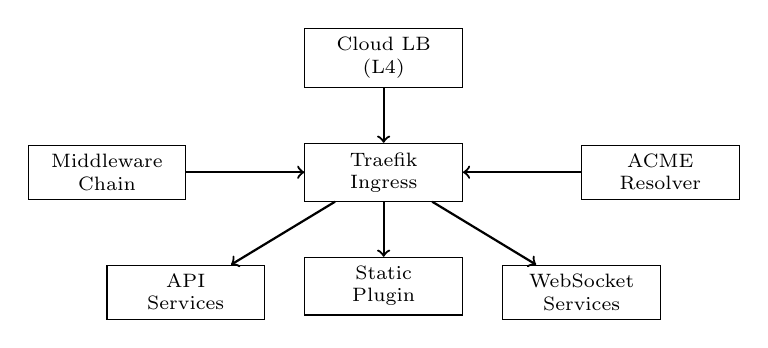
\begin{tikzpicture}[
    node distance=0.7cm,
    box/.style={rectangle, draw, minimum width=2cm, minimum height=0.5cm, align=center, font=\scriptsize},
    arrow/.style={->, thick}
]
\node[box] (lb) {Cloud LB\\(L4)};
\node[box, below=of lb] (traefik) {Traefik\\Ingress};
\node[box, below left=0.8cm and 0.5cm of traefik] (api) {API\\Services};
\node[box, below=of traefik] (static) {Static\\Plugin};
\node[box, below right=0.8cm and 0.5cm of traefik] (ws) {WebSocket\\Services};
\node[box, right=1.5cm of traefik] (acme) {ACME\\Resolver};
\node[box, left=1.5cm of traefik] (mw) {Middleware\\Chain};

\draw[arrow] (lb) -- (traefik);
\draw[arrow] (traefik) -- (api);
\draw[arrow] (traefik) -- (static);
\draw[arrow] (traefik) -- (ws);
\draw[arrow] (acme) -- (traefik);
\draw[arrow] (mw) -- (traefik);
\end{tikzpicture}
\caption{Ingress deployment with static plugin and ACME resolver.}
\label{fig:ingress}
\end{figure}

Hanzo Ingress runs as a DaemonSet on dedicated ingress nodes, behind a cloud Layer~4 load balancer (Figure~\ref{fig:ingress}). Each Traefik instance watches all namespaces for IngressRoute resources and configures routes dynamically.

\subsection{IngressRoute Configuration}

Routes are defined using Traefik's IngressRoute CRD:

\begin{lstlisting}[language=YAML]
apiVersion: traefik.io/v1alpha1
kind: IngressRoute
metadata:
  name: web-app
  namespace: production
spec:
  entryPoints: [websecure]
  routes:
  - match: Host(`app.hanzo.ai`)
    kind: Rule
    services:
    - name: web-app
      port: 8080
    middlewares:
    - name: security-headers
    - name: compress
  tls:
    certResolver: letsencrypt
\end{lstlisting}

\subsection{Static File Plugin}

The static file plugin serves files from a mounted volume, supporting SPA routing (fallback to \texttt{index.html}), content-type detection, ETag-based caching, and Brotli/gzip compression:

\begin{lstlisting}[language=YAML]
apiVersion: traefik.io/v1alpha1
kind: Middleware
metadata:
  name: static-files
spec:
  plugin:
    hanzo-static:
      root: /srv/web
      index: index.html
      spaFallback: true
      cacheControl: "public, max-age=31536000"
      immutablePrefix: "/assets/"
\end{lstlisting}

Files under \texttt{/assets/} receive immutable cache headers (1 year), while \texttt{index.html} receives \texttt{no-cache} to ensure users always load the latest version. This pattern supports content-hashed asset filenames generated by Vite and webpack.

\section{Key Features}

\subsection{Automatic TLS}

Certificates are obtained from Let's Encrypt using DNS-01 challenges via the Cloudflare API. This approach supports wildcard certificates (\texttt{*.hanzo.ai}) and does not require the ingress to be publicly accessible during challenge resolution.

Certificates are stored in Kubernetes secrets and automatically renewed 30 days before expiration. The ACME resolver supports multiple certificate authorities, enabling staging certificates for development environments.

\subsection{Middleware Chain}

Requests pass through an ordered middleware chain. Standard middleware includes:

\begin{itemize}
    \item \textbf{Security headers}: HSTS, X-Frame-Options, CSP, X-Content-Type-Options
    \item \textbf{Compression}: Brotli (preferred) and gzip
    \item \textbf{Rate limiting}: Per-IP with configurable burst
    \item \textbf{Auth forwarding}: Delegates to Hanzo IAM for protected routes
    \item \textbf{Strip prefix}: Removes path prefixes before forwarding
    \item \textbf{Retry}: Automatic retry on 502/503 with exponential backoff
\end{itemize}

\subsection{Multi-Namespace Routing}

Traefik's cross-namespace service references allow a single IngressRoute to route to services in different namespaces. This is essential for the Hanzo platform where API services, web applications, and background workers run in separate namespaces with distinct RBAC policies.

\section{Implementation}

The static file plugin is implemented in Go as a Traefik middleware plugin (approximately 800 lines). It uses \texttt{http.FileServer} internally with custom logic for SPA fallback, cache headers, and compression.

\paragraph{Resource Usage.} Memory and CPU scale with the number of live connections and the size of the routing table rather than with request rate, since neither TLS session state nor the static-file cache is per-request. Concrete figures for a named workload are not reported here (Section~\ref{sec:figures}).

\section{Status of the performance figures}
\label{sec:figures}

An earlier version of this paper carried a table titled ``Latency overhead
comparison (ms, p99)'' placing Hanzo Ingress at 1.2\,ms on an API route and
0.8\,ms on a static file against 1.8/2.2\,ms for nginx with a sidecar and
1.5/1.8\,ms for Caddy, and an abstract claiming a 40\% reduction in pod count.

None of it was measured. The comparison named no load generator, no hardware, no
request count and no configuration for either competitor, which makes it a claim
about two third-party products with nothing behind it --- the most exposed kind
of number a paper can carry. The 40\% figure defined neither ``typical
deployment'' nor a before-and-after pod inventory. Both are removed.

The structural argument the table was meant to support does not need it: serving
a static asset from the ingress rather than from a pod behind it removes a
network hop and a container from the path. That is a statement about the
topology, and it holds whatever the measured difference turns out to be.

A sidecar-based approach pays for a second process and the hop to reach it on every static request. The plugin serves the file from the process that already terminated the connection, so neither cost appears.

\section{Security}

\paragraph{TLS Configuration.} Only TLS~1.2 and 1.3 are supported. Cipher suites are restricted to AEAD ciphers (AES-GCM, ChaCha20-Poly1305). HSTS is enabled with a 1-year max-age and includeSubDomains.

\paragraph{Certificate Security.} Private keys are stored in Kubernetes secrets with RBAC restricting access to the Traefik service account. Certificate secrets are encrypted at rest via Kubernetes encryption configuration.

\paragraph{Request Filtering.} Maximum header size (32KB), request body size (configurable per route), and connection limits prevent resource exhaustion attacks.

\paragraph{Network Policy.} Ingress pods accept traffic only from the cloud load balancer CIDR. Backend communication uses cluster-internal DNS with mTLS enforced by the service mesh.

\section{Conclusion}

Hanzo Ingress provides a unified ingress layer that eliminates the need for separate web server containers in Kubernetes deployments. The static file plugin serves SPAs and assets directly from the ingress controller, which removes a container and a hop from the path an asset takes. Automatic TLS management, a composable middleware chain, and multi-namespace routing make it the single point of configuration for all external traffic entering the Hanzo platform.

\bibliographystyle{plain}
\begin{thebibliography}{10}

\bibitem{traefik2016}
Traefik Labs. Traefik: The Cloud Native Application Proxy. 2016.

\bibitem{letsencrypt2015}
J. Aas et al. Let's Encrypt: A Free, Automated, and Open Certificate Authority. ACM CCS, 2019.

\bibitem{kubernetes2015}
B. Burns et al. Borg, Omega, and Kubernetes. ACM Queue, 2016.

\end{thebibliography}

\end{document}
